\documentclass[1p]{elsarticle_modified}
%\bibliographystyle{elsarticle-num}

%\usepackage[colorlinks]{hyperref}
%\usepackage{abbrmath_seonhwa} %\Abb, \Ascr, \Acal ,\Abf, \Afrak
\usepackage{amsfonts}
\usepackage{amssymb}
\usepackage{amsmath}
\usepackage{amsthm}
\usepackage{scalefnt}
\usepackage{amsbsy}
\usepackage{kotex}
\usepackage{caption}
\usepackage{subfig}
\usepackage{color}
\usepackage{graphicx}
\usepackage{xcolor} %% white, black, red, green, blue, cyan, magenta, yellow
\usepackage{float}
\usepackage{setspace}
\usepackage{hyperref}

\usepackage{tikz}
\usetikzlibrary{arrows}

\usepackage{multirow}
\usepackage{array} % fixed length table
\usepackage{hhline}

%%%%%%%%%%%%%%%%%%%%%
\makeatletter
\renewcommand*\env@matrix[1][\arraystretch]{%
	\edef\arraystretch{#1}%
	\hskip -\arraycolsep
	\let\@ifnextchar\new@ifnextchar
	\array{*\c@MaxMatrixCols c}}
\makeatother %https://tex.stackexchange.com/questions/14071/how-can-i-increase-the-line-spacing-in-a-matrix
%%%%%%%%%%%%%%%

\usepackage[normalem]{ulem}

\newcommand{\msout}[1]{\ifmmode\text{\sout{\ensuremath{#1}}}\else\sout{#1}\fi}
%SOURCE: \msout is \stkout macro in https://tex.stackexchange.com/questions/20609/strikeout-in-math-mode

\newcommand{\cancel}[1]{
	\ifmmode
	{\color{red}\msout{#1}}
	\else
	{\color{red}\sout{#1}}
	\fi
}

\newcommand{\add}[1]{
	{\color{blue}\uwave{#1}}
}

\newcommand{\replace}[2]{
	\ifmmode
	{\color{red}\msout{#1}}{\color{blue}\uwave{#2}}
	\else
	{\color{red}\sout{#1}}{\color{blue}\uwave{#2}}
	\fi
}

\newcommand{\Sol}{\mathcal{S}} %segment
\newcommand{\D}{D} %diagram
\newcommand{\A}{\mathcal{A}} %arc


%%%%%%%%%%%%%%%%%%%%%%%%%%%%%5 test

\def\sl{\operatorname{\textup{SL}}(2,\Cbb)}
\def\psl{\operatorname{\textup{PSL}}(2,\Cbb)}
\def\quan{\mkern 1mu \triangleright \mkern 1mu}

\theoremstyle{definition}
\newtheorem{thm}{Theorem}[section]
\newtheorem{prop}[thm]{Proposition}
\newtheorem{lem}[thm]{Lemma}
\newtheorem{ques}[thm]{Question}
\newtheorem{cor}[thm]{Corollary}
\newtheorem{defn}[thm]{Definition}
\newtheorem{exam}[thm]{Example}
\newtheorem{rmk}[thm]{Remark}
\newtheorem{alg}[thm]{Algorithm}

\newcommand{\I}{\sqrt{-1}}
\begin{document}

%\begin{frontmatter}
%
%\title{Boundary parabolic representations of knots up to 8 crossings}
%
%%% Group authors per affiliation:
%\author{Yunhi Cho} 
%\address{Department of Mathematics, University of Seoul, Seoul, Korea}
%\ead{yhcho@uos.ac.kr}
%
%
%\author{Seonhwa Kim} %\fnref{s_kim}}
%\address{Center for Geometry and Physics, Institute for Basic Science, Pohang, 37673, Korea}
%\ead{ryeona17@ibs.re.kr}
%
%\author{Hyuk Kim}
%\address{Department of Mathematical Sciences, Seoul National University, Seoul 08826, Korea}
%\ead{hyukkim@snu.ac.kr}
%
%\author{Seokbeom Yoon}
%\address{Department of Mathematical Sciences, Seoul National University, Seoul, 08826,  Korea}
%\ead{sbyoon15@snu.ac.kr}
%
%\begin{abstract}
%We find all boundary parabolic representation of knots up to 8 crossings.
%
%\end{abstract}
%\begin{keyword}
%    \MSC[2010] 57M25 
%\end{keyword}
%
%\end{frontmatter}

%\linenumbers
%\tableofcontents
%
\newcommand\colored[1]{\textcolor{white}{\rule[-0.35ex]{0.8em}{1.4ex}}\kern-0.8em\color{red} #1}%
%\newcommand\colored[1]{\textcolor{white}{ #1}\kern-2.17ex	\textcolor{white}{ #1}\kern-1.81ex	\textcolor{white}{ #1}\kern-2.15ex\color{red}#1	}

{\Large $\underline{12a_{0251}~(K12a_{0251})}$}

\setlength{\tabcolsep}{10pt}
\renewcommand{\arraystretch}{1.6}
\vspace{1cm}\begin{tabular}{m{100pt}>{\centering\arraybackslash}m{274pt}}
\multirow{5}{120pt}{
	\centering
	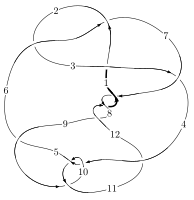
\includegraphics[width=112pt]{../../../GIT/diagram.site/Diagrams/png/1052_12a_0251.png}\\
\ \ \ A knot diagram\footnotemark}&
\allowdisplaybreaks
\textbf{Linearized knot diagam} \\
\cline{2-2}
 &
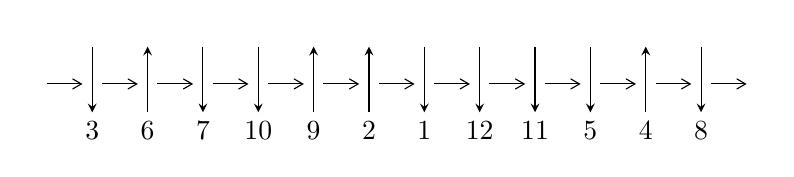
\begin{tikzpicture}[x=20pt, y=17pt]
	% nodes
	\node (C0) at (0, 0) {};
	\node (C1) at (1, 0) {};
	\node (C1U) at (1, +1) {};
	\node (C1D) at (1, -1) {3};

	\node (C2) at (2, 0) {};
	\node (C2U) at (2, +1) {};
	\node (C2D) at (2, -1) {6};

	\node (C3) at (3, 0) {};
	\node (C3U) at (3, +1) {};
	\node (C3D) at (3, -1) {7};

	\node (C4) at (4, 0) {};
	\node (C4U) at (4, +1) {};
	\node (C4D) at (4, -1) {10};

	\node (C5) at (5, 0) {};
	\node (C5U) at (5, +1) {};
	\node (C5D) at (5, -1) {9};

	\node (C6) at (6, 0) {};
	\node (C6U) at (6, +1) {};
	\node (C6D) at (6, -1) {2};

	\node (C7) at (7, 0) {};
	\node (C7U) at (7, +1) {};
	\node (C7D) at (7, -1) {1};

	\node (C8) at (8, 0) {};
	\node (C8U) at (8, +1) {};
	\node (C8D) at (8, -1) {12};

	\node (C9) at (9, 0) {};
	\node (C9U) at (9, +1) {};
	\node (C9D) at (9, -1) {11};

	\node (C10) at (10, 0) {};
	\node (C10U) at (10, +1) {};
	\node (C10D) at (10, -1) {5};

	\node (C11) at (11, 0) {};
	\node (C11U) at (11, +1) {};
	\node (C11D) at (11, -1) {4};

	\node (C12) at (12, 0) {};
	\node (C12U) at (12, +1) {};
	\node (C12D) at (12, -1) {8};
	\node (C13) at (13, 0) {};

	% arrows
	\draw[->,>={angle 60}]
	(C0) edge (C1) (C1) edge (C2) (C2) edge (C3) (C3) edge (C4) (C4) edge (C5) (C5) edge (C6) (C6) edge (C7) (C7) edge (C8) (C8) edge (C9) (C9) edge (C10) (C10) edge (C11) (C11) edge (C12) (C12) edge (C13) ;	\draw[->,>=stealth]
	(C1U) edge (C1D) (C2D) edge (C2U) (C3U) edge (C3D) (C4U) edge (C4D) (C5D) edge (C5U) (C6D) edge (C6U) (C7U) edge (C7D) (C8U) edge (C8D) (C9U) edge (C9D) (C10U) edge (C10D) (C11D) edge (C11U) (C12U) edge (C12D) ;
	\end{tikzpicture} \\
\hhline{~~} \\& 
\textbf{Solving Sequence} \\ \cline{2-2} 
 &
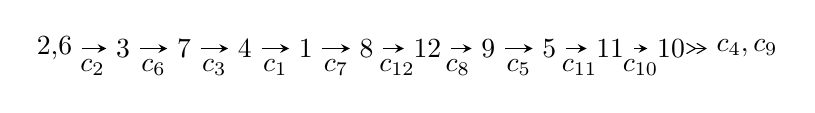
\begin{tikzpicture}[x=22pt, y=7pt]
	% node
	\node (A0) at (-1/8, 0) {2,6};
	\node (A1) at (1, 0) {3};
	\node (A2) at (2, 0) {7};
	\node (A3) at (3, 0) {4};
	\node (A4) at (4, 0) {1};
	\node (A5) at (5, 0) {8};
	\node (A6) at (6, 0) {12};
	\node (A7) at (7, 0) {9};
	\node (A8) at (8, 0) {5};
	\node (A9) at (9, 0) {11};
	\node (A10) at (10, 0) {10};
	\node (C1) at (1/2, -1) {$c_{2}$};
	\node (C2) at (3/2, -1) {$c_{6}$};
	\node (C3) at (5/2, -1) {$c_{3}$};
	\node (C4) at (7/2, -1) {$c_{1}$};
	\node (C5) at (9/2, -1) {$c_{7}$};
	\node (C6) at (11/2, -1) {$c_{12}$};
	\node (C7) at (13/2, -1) {$c_{8}$};
	\node (C8) at (15/2, -1) {$c_{5}$};
	\node (C9) at (17/2, -1) {$c_{11}$};
	\node (C10) at (19/2, -1) {$c_{10}$};
	\node (A11) at (45/4, 0) {$c_{4},c_{9}$};

	% edge
	\draw[->,>=stealth]	
	(A0) edge (A1) (A1) edge (A2) (A2) edge (A3) (A3) edge (A4) (A4) edge (A5) (A5) edge (A6) (A6) edge (A7) (A7) edge (A8) (A8) edge (A9) (A9) edge (A10) ;
	\draw[->>,>={angle 60}]	
	(A10) edge (A11);
\end{tikzpicture} \\ 

\end{tabular} \\

\footnotetext{
The image of knot diagram is generated by the software ``\textbf{Draw programme}" developed by Andrew Bartholomew(\url{http://www.layer8.co.uk/maths/draw/index.htm\#Running-draw}), where we modified some parts for our purpose(\url{https://github.com/CATsTAILs/LinksPainter}).
}\phantom \\ \newline 
\centering \textbf{Ideals for irreducible components\footnotemark of $X_{\text{par}}$} 
 
\begin{align*}
I^u_{1}&=\langle 
u^{79}- u^{78}+\cdots+4 u^3+1\rangle \\
\\
\end{align*}
\raggedright * 1 irreducible components of $\dim_{\mathbb{C}}=0$, with total 79 representations.\\
\footnotetext{All coefficients of polynomials are rational numbers. But the coefficients are sometimes approximated in decimal forms when there is not enough margin.}
\newpage
\renewcommand{\arraystretch}{1}
\centering \section*{I. $I^u_{1}= \langle u^{79}- u^{78}+\cdots+4 u^3+1 \rangle$}
\flushleft \textbf{(i) Arc colorings}\\
\begin{tabular}{m{7pt} m{180pt} m{7pt} m{180pt} }
\flushright $a_{2}=$&$\begin{pmatrix}1\\0\end{pmatrix}$ \\
\flushright $a_{6}=$&$\begin{pmatrix}0\\u\end{pmatrix}$ \\
\flushright $a_{3}=$&$\begin{pmatrix}1\\- u^2\end{pmatrix}$ \\
\flushright $a_{7}=$&$\begin{pmatrix}u\\u\end{pmatrix}$ \\
\flushright $a_{4}=$&$\begin{pmatrix}u^4+u^2+1\\u^4\end{pmatrix}$ \\
\flushright $a_{1}=$&$\begin{pmatrix}u^2+1\\- u^4\end{pmatrix}$ \\
\flushright $a_{8}=$&$\begin{pmatrix}- u^7-2 u^5-2 u^3\\u^9+u^7+u^5+u\end{pmatrix}$ \\
\flushright $a_{12}=$&$\begin{pmatrix}u^{12}+3 u^{10}+5 u^8+4 u^6+2 u^4+u^2+1\\- u^{14}-2 u^{12}-3 u^{10}-2 u^8-2 u^6-2 u^4- u^2\end{pmatrix}$ \\
\flushright $a_{9}=$&$\begin{pmatrix}- u^{17}-4 u^{15}-9 u^{13}-12 u^{11}-11 u^9-8 u^7-6 u^5-4 u^3- u\\u^{19}+3 u^{17}+6 u^{15}+7 u^{13}+7 u^{11}+7 u^9+6 u^7+4 u^5+u^3+u\end{pmatrix}$ \\
\flushright $a_{5}=$&$\begin{pmatrix}- u^{35}-8 u^{33}+\cdots-8 u^5- u^3\\u^{37}+7 u^{35}+\cdots+u^3+u\end{pmatrix}$ \\
\flushright $a_{11}=$&$\begin{pmatrix}u^{22}+5 u^{20}+\cdots+2 u^2+1\\u^{22}+4 u^{20}+9 u^{18}+12 u^{16}+10 u^{14}+6 u^{12}+3 u^{10}+2 u^8- u^6-2 u^4- u^2\end{pmatrix}$ \\
\flushright $a_{10}=$&$\begin{pmatrix}- u^{63}-14 u^{61}+\cdots-8 u^3-2 u\\- u^{63}-13 u^{61}+\cdots+2 u^3+u\end{pmatrix}$\\&\end{tabular}
\flushleft \textbf{(ii) Obstruction class $= -1$}\\~\\
\flushleft \textbf{(iii) Cusp Shapes $= -4 u^{78}+4 u^{77}+\cdots-8 u^2-2$}\\~\\
\newpage\renewcommand{\arraystretch}{1}
\flushleft \textbf{(iv) u-Polynomials at the component}\newline \\
\begin{tabular}{m{50pt}|m{274pt}}
Crossings & \hspace{64pt}u-Polynomials at each crossing \\
\hline $$\begin{aligned}c_{1}\end{aligned}$$&$\begin{aligned}
&u^{79}+35 u^{78}+\cdots+8 u^2-1
\end{aligned}$\\
\hline $$\begin{aligned}c_{2},c_{6}\end{aligned}$$&$\begin{aligned}
&u^{79}- u^{78}+\cdots+4 u^3+1
\end{aligned}$\\
\hline $$\begin{aligned}c_{3}\end{aligned}$$&$\begin{aligned}
&u^{79}+u^{78}+\cdots+9 u+2
\end{aligned}$\\
\hline $$\begin{aligned}c_{4},c_{10}\end{aligned}$$&$\begin{aligned}
&u^{79}- u^{78}+\cdots-2 u^4+1
\end{aligned}$\\
\hline $$\begin{aligned}c_{5},c_{11}\end{aligned}$$&$\begin{aligned}
&u^{79}-3 u^{78}+\cdots-445 u+88
\end{aligned}$\\
\hline $$\begin{aligned}c_{7},c_{8},c_{12}\end{aligned}$$&$\begin{aligned}
&u^{79}-5 u^{78}+\cdots-24 u+1
\end{aligned}$\\
\hline $$\begin{aligned}c_{9}\end{aligned}$$&$\begin{aligned}
&u^{79}+41 u^{78}+\cdots-4 u^2+1
\end{aligned}$\\
\hline
\end{tabular}\\~\\
\newpage\renewcommand{\arraystretch}{1}
\flushleft \textbf{(v) Riley Polynomials at the component}\newline \\
\begin{tabular}{m{50pt}|m{274pt}}
Crossings & \hspace{64pt}Riley Polynomials at each crossing \\
\hline $$\begin{aligned}c_{1}\end{aligned}$$&$\begin{aligned}
&y^{79}+19 y^{78}+\cdots+16 y-1
\end{aligned}$\\
\hline $$\begin{aligned}c_{2},c_{6}\end{aligned}$$&$\begin{aligned}
&y^{79}+35 y^{78}+\cdots+8 y^2-1
\end{aligned}$\\
\hline $$\begin{aligned}c_{3}\end{aligned}$$&$\begin{aligned}
&y^{79}+3 y^{78}+\cdots-139 y-4
\end{aligned}$\\
\hline $$\begin{aligned}c_{4},c_{10}\end{aligned}$$&$\begin{aligned}
&y^{79}-41 y^{78}+\cdots+4 y^2-1
\end{aligned}$\\
\hline $$\begin{aligned}c_{5},c_{11}\end{aligned}$$&$\begin{aligned}
&y^{79}+51 y^{78}+\cdots+140825 y-7744
\end{aligned}$\\
\hline $$\begin{aligned}c_{7},c_{8},c_{12}\end{aligned}$$&$\begin{aligned}
&y^{79}+79 y^{78}+\cdots+72 y-1
\end{aligned}$\\
\hline $$\begin{aligned}c_{9}\end{aligned}$$&$\begin{aligned}
&y^{79}-5 y^{78}+\cdots+8 y-1
\end{aligned}$\\
\hline
\end{tabular}\\~\\
\newpage\flushleft \textbf{(vi) Complex Volumes and Cusp Shapes}
$$\begin{array}{c|c|c}  
\text{Solutions to }I^u_{1}& \I (\text{vol} + \sqrt{-1}CS) & \text{Cusp shape}\\
 \hline 
\begin{aligned}
u &= -0.518439 + 0.839977 I\end{aligned}
 & -2.47695 + 1.61220 I & \phantom{-0.000000 } 0 \\ \hline\begin{aligned}
u &= -0.518439 - 0.839977 I\end{aligned}
 & -2.47695 - 1.61220 I & \phantom{-0.000000 } 0 \\ \hline\begin{aligned}
u &= -0.250874 + 0.935800 I\end{aligned}
 & -2.18929 + 0.78848 I & -9.38930 - 3.30417 I \\ \hline\begin{aligned}
u &= -0.250874 - 0.935800 I\end{aligned}
 & -2.18929 - 0.78848 I & -9.38930 + 3.30417 I \\ \hline\begin{aligned}
u &= \phantom{-}0.472540 + 0.928709 I\end{aligned}
 & -0.19704 + 2.19503 I & \phantom{-0.000000 } 0 \\ \hline\begin{aligned}
u &= \phantom{-}0.472540 - 0.928709 I\end{aligned}
 & -0.19704 - 2.19503 I & \phantom{-0.000000 } 0 \\ \hline\begin{aligned}
u &= -0.777679 + 0.521809 I\end{aligned}
 & \phantom{-}3.79637 - 7.20850 I & -1.29301 + 5.78914 I \\ \hline\begin{aligned}
u &= -0.777679 - 0.521809 I\end{aligned}
 & \phantom{-}3.79637 + 7.20850 I & -1.29301 - 5.78914 I \\ \hline\begin{aligned}
u &= \phantom{-}0.790583 + 0.491775 I\end{aligned}
 & \phantom{-}8.97318 + 0.79076 I & \phantom{-}3.03187 - 3.00040 I \\ \hline\begin{aligned}
u &= \phantom{-}0.790583 - 0.491775 I\end{aligned}
 & \phantom{-}8.97318 - 0.79076 I & \phantom{-}3.03187 + 3.00040 I \\ \hline\begin{aligned}
u &= \phantom{-}0.776695 + 0.512527 I\end{aligned}
 & \phantom{-}6.49253 + 2.31855 I & \phantom{-}1.93099 - 2.22263 I \\ \hline\begin{aligned}
u &= \phantom{-}0.776695 - 0.512527 I\end{aligned}
 & \phantom{-}6.49253 - 2.31855 I & \phantom{-}1.93099 + 2.22263 I \\ \hline\begin{aligned}
u &= -0.794225 + 0.480848 I\end{aligned}
 & \phantom{-}8.91071 + 3.99166 I & \phantom{-}2.81554 - 3.57592 I \\ \hline\begin{aligned}
u &= -0.794225 - 0.480848 I\end{aligned}
 & \phantom{-}8.91071 - 3.99166 I & \phantom{-}2.81554 + 3.57592 I \\ \hline\begin{aligned}
u &= \phantom{-}0.799974 + 0.452152 I\end{aligned}
 & \phantom{-}3.40222 - 10.36420 I & -1.86089 + 6.02560 I \\ \hline\begin{aligned}
u &= \phantom{-}0.799974 - 0.452152 I\end{aligned}
 & \phantom{-}3.40222 + 10.36420 I & -1.86089 - 6.02560 I \\ \hline\begin{aligned}
u &= -0.795010 + 0.457768 I\end{aligned}
 & \phantom{-}6.18261 + 5.44195 I & \phantom{-}1.37667 - 2.61754 I \\ \hline\begin{aligned}
u &= -0.795010 - 0.457768 I\end{aligned}
 & \phantom{-}6.18261 - 5.44195 I & \phantom{-}1.37667 + 2.61754 I \\ \hline\begin{aligned}
u &= -0.539580 + 0.740555 I\end{aligned}
 & -2.19284 - 5.95136 I & -3.06972 + 7.35183 I \\ \hline\begin{aligned}
u &= -0.539580 - 0.740555 I\end{aligned}
 & -2.19284 + 5.95136 I & -3.06972 - 7.35183 I \\ \hline\begin{aligned}
u &= \phantom{-}0.078728 + 1.082670 I\end{aligned}
 & -3.31194 - 0.08407 I & \phantom{-0.000000 } 0 \\ \hline\begin{aligned}
u &= \phantom{-}0.078728 - 1.082670 I\end{aligned}
 & -3.31194 + 0.08407 I & \phantom{-0.000000 } 0 \\ \hline\begin{aligned}
u &= -0.758214 + 0.509308 I\end{aligned}
 & \phantom{-}2.23994 + 0.99895 I & -3.29257 - 0.53289 I \\ \hline\begin{aligned}
u &= -0.758214 - 0.509308 I\end{aligned}
 & \phantom{-}2.23994 - 0.99895 I & -3.29257 + 0.53289 I \\ \hline\begin{aligned}
u &= \phantom{-}0.782931 + 0.451118 I\end{aligned}
 & \phantom{-}1.90919 - 1.95514 I & -3.75115 + 0. I\phantom{ +0.000000I} \\ \hline\begin{aligned}
u &= \phantom{-}0.782931 - 0.451118 I\end{aligned}
 & \phantom{-}1.90919 + 1.95514 I & -3.75115 + 0. I\phantom{ +0.000000I} \\ \hline\begin{aligned}
u &= -0.057574 + 1.102150 I\end{aligned}
 & \phantom{-}0.80009 + 3.56647 I & \phantom{-0.000000 } 0 \\ \hline\begin{aligned}
u &= -0.057574 - 1.102150 I\end{aligned}
 & \phantom{-}0.80009 - 3.56647 I & \phantom{-0.000000 } 0 \\ \hline\begin{aligned}
u &= -0.011598 + 1.103820 I\end{aligned}
 & \phantom{-}3.36202 + 2.32895 I & \phantom{-0.000000 } 0 \\ \hline\begin{aligned}
u &= -0.011598 - 1.103820 I\end{aligned}
 & \phantom{-}3.36202 - 2.32895 I & \phantom{-0.000000 } 0\\
 \hline 
 \end{array}$$\newpage$$\begin{array}{c|c|c}  
\text{Solutions to }I^u_{1}& \I (\text{vol} + \sqrt{-1}CS) & \text{Cusp shape}\\
 \hline 
\begin{aligned}
u &= -0.330330 + 1.053940 I\end{aligned}
 & -4.29872 - 0.60827 I & \phantom{-0.000000 } 0 \\ \hline\begin{aligned}
u &= -0.330330 - 1.053940 I\end{aligned}
 & -4.29872 + 0.60827 I & \phantom{-0.000000 } 0 \\ \hline\begin{aligned}
u &= \phantom{-}0.315571 + 1.069460 I\end{aligned}
 & -7.52343 - 3.77517 I & \phantom{-0.000000 } 0 \\ \hline\begin{aligned}
u &= \phantom{-}0.315571 - 1.069460 I\end{aligned}
 & -7.52343 + 3.77517 I & \phantom{-0.000000 } 0 \\ \hline\begin{aligned}
u &= \phantom{-}0.066591 + 1.113330 I\end{aligned}
 & -1.99034 - 8.40432 I & \phantom{-0.000000 } 0 \\ \hline\begin{aligned}
u &= \phantom{-}0.066591 - 1.113330 I\end{aligned}
 & -1.99034 + 8.40432 I & \phantom{-0.000000 } 0 \\ \hline\begin{aligned}
u &= \phantom{-}0.518854 + 0.988102 I\end{aligned}
 & \phantom{-}0.41468 + 2.88353 I & \phantom{-0.000000 } 0 \\ \hline\begin{aligned}
u &= \phantom{-}0.518854 - 0.988102 I\end{aligned}
 & \phantom{-}0.41468 - 2.88353 I & \phantom{-0.000000 } 0 \\ \hline\begin{aligned}
u &= -0.430212 + 1.031220 I\end{aligned}
 & -3.49022 - 3.24568 I & \phantom{-0.000000 } 0 \\ \hline\begin{aligned}
u &= -0.430212 - 1.031220 I\end{aligned}
 & -3.49022 + 3.24568 I & \phantom{-0.000000 } 0 \\ \hline\begin{aligned}
u &= \phantom{-}0.345422 + 1.071560 I\end{aligned}
 & -7.79780 + 4.70521 I & \phantom{-0.000000 } 0 \\ \hline\begin{aligned}
u &= \phantom{-}0.345422 - 1.071560 I\end{aligned}
 & -7.79780 - 4.70521 I & \phantom{-0.000000 } 0 \\ \hline\begin{aligned}
u &= \phantom{-}0.472065 + 0.706972 I\end{aligned}
 & \phantom{-}0.43948 + 1.74919 I & \phantom{-}0.70667 - 4.05874 I \\ \hline\begin{aligned}
u &= \phantom{-}0.472065 - 0.706972 I\end{aligned}
 & \phantom{-}0.43948 - 1.74919 I & \phantom{-}0.70667 + 4.05874 I \\ \hline\begin{aligned}
u &= -0.530932 + 1.032320 I\end{aligned}
 & -0.41303 - 6.78330 I & \phantom{-0.000000 } 0 \\ \hline\begin{aligned}
u &= -0.530932 - 1.032320 I\end{aligned}
 & -0.41303 + 6.78330 I & \phantom{-0.000000 } 0 \\ \hline\begin{aligned}
u &= -0.498801 + 1.079610 I\end{aligned}
 & -3.17706 - 6.37439 I & \phantom{-0.000000 } 0 \\ \hline\begin{aligned}
u &= -0.498801 - 1.079610 I\end{aligned}
 & -3.17706 + 6.37439 I & \phantom{-0.000000 } 0 \\ \hline\begin{aligned}
u &= \phantom{-}0.484264 + 1.086440 I\end{aligned}
 & -6.87950 + 2.43282 I & \phantom{-0.000000 } 0 \\ \hline\begin{aligned}
u &= \phantom{-}0.484264 - 1.086440 I\end{aligned}
 & -6.87950 - 2.43282 I & \phantom{-0.000000 } 0 \\ \hline\begin{aligned}
u &= \phantom{-}0.503668 + 1.090740 I\end{aligned}
 & -6.28401 + 10.93530 I & \phantom{-0.000000 } 0 \\ \hline\begin{aligned}
u &= \phantom{-}0.503668 - 1.090740 I\end{aligned}
 & -6.28401 - 10.93530 I & \phantom{-0.000000 } 0 \\ \hline\begin{aligned}
u &= -0.615780 + 1.056650 I\end{aligned}
 & \phantom{-}0.60926 - 6.20761 I & \phantom{-0.000000 } 0 \\ \hline\begin{aligned}
u &= -0.615780 - 1.056650 I\end{aligned}
 & \phantom{-}0.60926 + 6.20761 I & \phantom{-0.000000 } 0 \\ \hline\begin{aligned}
u &= -0.631557 + 1.055390 I\end{aligned}
 & \phantom{-}2.20395 + 1.89316 I & \phantom{-0.000000 } 0 \\ \hline\begin{aligned}
u &= -0.631557 - 1.055390 I\end{aligned}
 & \phantom{-}2.20395 - 1.89316 I & \phantom{-0.000000 } 0 \\ \hline\begin{aligned}
u &= \phantom{-}0.627875 + 1.060360 I\end{aligned}
 & \phantom{-}4.85794 + 2.98135 I & \phantom{-0.000000 } 0 \\ \hline\begin{aligned}
u &= \phantom{-}0.627875 - 1.060360 I\end{aligned}
 & \phantom{-}4.85794 - 2.98135 I & \phantom{-0.000000 } 0 \\ \hline\begin{aligned}
u &= \phantom{-}0.628251 + 1.075530 I\end{aligned}
 & \phantom{-}7.22967 + 4.54653 I & \phantom{-0.000000 } 0 \\ \hline\begin{aligned}
u &= \phantom{-}0.628251 - 1.075530 I\end{aligned}
 & \phantom{-}7.22967 - 4.54653 I & \phantom{-0.000000 } 0\\
 \hline 
 \end{array}$$\newpage$$\begin{array}{c|c|c}  
\text{Solutions to }I^u_{1}& \I (\text{vol} + \sqrt{-1}CS) & \text{Cusp shape}\\
 \hline 
\begin{aligned}
u &= -0.626429 + 1.081980 I\end{aligned}
 & \phantom{-}7.11532 - 9.33149 I & \phantom{-0.000000 } 0 \\ \hline\begin{aligned}
u &= -0.626429 - 1.081980 I\end{aligned}
 & \phantom{-}7.11532 + 9.33149 I & \phantom{-0.000000 } 0 \\ \hline\begin{aligned}
u &= \phantom{-}0.612337 + 1.091520 I\end{aligned}
 & \phantom{-}0.00350 + 7.21255 I & \phantom{-0.000000 } 0 \\ \hline\begin{aligned}
u &= \phantom{-}0.612337 - 1.091520 I\end{aligned}
 & \phantom{-}0.00350 - 7.21255 I & \phantom{-0.000000 } 0 \\ \hline\begin{aligned}
u &= \phantom{-}0.516957 + 0.538342 I\end{aligned}
 & \phantom{-}1.69269 + 1.37789 I & \phantom{-}2.70355 - 4.03268 I \\ \hline\begin{aligned}
u &= \phantom{-}0.516957 - 0.538342 I\end{aligned}
 & \phantom{-}1.69269 - 1.37789 I & \phantom{-}2.70355 + 4.03268 I \\ \hline\begin{aligned}
u &= -0.619167 + 1.092530 I\end{aligned}
 & \phantom{-}4.28876 - 10.75590 I & \phantom{-0.000000 } 0 \\ \hline\begin{aligned}
u &= -0.619167 - 1.092530 I\end{aligned}
 & \phantom{-}4.28876 + 10.75590 I & \phantom{-0.000000 } 0 \\ \hline\begin{aligned}
u &= \phantom{-}0.619393 + 1.096430 I\end{aligned}
 & \phantom{-}1.4791 + 15.6911 I & \phantom{-0.000000 } 0 \\ \hline\begin{aligned}
u &= \phantom{-}0.619393 - 1.096430 I\end{aligned}
 & \phantom{-}1.4791 - 15.6911 I & \phantom{-0.000000 } 0 \\ \hline\begin{aligned}
u &= -0.560028 + 0.413582 I\end{aligned}
 & \phantom{-}1.30119 + 2.38830 I & \phantom{-}0.66864 - 5.36145 I \\ \hline\begin{aligned}
u &= -0.560028 - 0.413582 I\end{aligned}
 & \phantom{-}1.30119 - 2.38830 I & \phantom{-}0.66864 + 5.36145 I \\ \hline\begin{aligned}
u &= \phantom{-}0.624420 + 0.239874 I\end{aligned}
 & -3.92703 - 6.58068 I & -5.74395 + 6.54636 I \\ \hline\begin{aligned}
u &= \phantom{-}0.624420 - 0.239874 I\end{aligned}
 & -3.92703 + 6.58068 I & -5.74395 - 6.54636 I \\ \hline\begin{aligned}
u &= -0.582840 + 0.243162 I\end{aligned}
 & -0.90156 + 2.12687 I & -2.58208 - 3.56451 I \\ \hline\begin{aligned}
u &= -0.582840 - 0.243162 I\end{aligned}
 & -0.90156 - 2.12687 I & -2.58208 + 3.56451 I \\ \hline\begin{aligned}
u &= \phantom{-}0.590316 + 0.185482 I\end{aligned}
 & -4.44704 + 1.71932 I & -7.28622 - 0.52322 I \\ \hline\begin{aligned}
u &= \phantom{-}0.590316 - 0.185482 I\end{aligned}
 & -4.44704 - 1.71932 I & -7.28622 + 0.52322 I \\ \hline\begin{aligned}
u &= -0.396331\phantom{ +0.000000I}\end{aligned}
 & -1.15940\phantom{ +0.000000I} & -8.74740\phantom{ +0.000000I}\\
 \hline 
 \end{array}$$\newpage
\newpage\renewcommand{\arraystretch}{1}
\centering \section*{ II. u-Polynomials}
\begin{tabular}{m{50pt}|m{274pt}}
Crossings & \hspace{64pt}u-Polynomials at each crossing \\
\hline $$\begin{aligned}c_{1}\end{aligned}$$&$\begin{aligned}
&u^{79}+35 u^{78}+\cdots+8 u^2-1
\end{aligned}$\\
\hline $$\begin{aligned}c_{2},c_{6}\end{aligned}$$&$\begin{aligned}
&u^{79}- u^{78}+\cdots+4 u^3+1
\end{aligned}$\\
\hline $$\begin{aligned}c_{3}\end{aligned}$$&$\begin{aligned}
&u^{79}+u^{78}+\cdots+9 u+2
\end{aligned}$\\
\hline $$\begin{aligned}c_{4},c_{10}\end{aligned}$$&$\begin{aligned}
&u^{79}- u^{78}+\cdots-2 u^4+1
\end{aligned}$\\
\hline $$\begin{aligned}c_{5},c_{11}\end{aligned}$$&$\begin{aligned}
&u^{79}-3 u^{78}+\cdots-445 u+88
\end{aligned}$\\
\hline $$\begin{aligned}c_{7},c_{8},c_{12}\end{aligned}$$&$\begin{aligned}
&u^{79}-5 u^{78}+\cdots-24 u+1
\end{aligned}$\\
\hline $$\begin{aligned}c_{9}\end{aligned}$$&$\begin{aligned}
&u^{79}+41 u^{78}+\cdots-4 u^2+1
\end{aligned}$\\
\hline
\end{tabular}\newpage\renewcommand{\arraystretch}{1}
\centering \section*{ III. Riley Polynomials}
\begin{tabular}{m{50pt}|m{274pt}}
Crossings & \hspace{64pt}Riley Polynomials at each crossing \\
\hline $$\begin{aligned}c_{1}\end{aligned}$$&$\begin{aligned}
&y^{79}+19 y^{78}+\cdots+16 y-1
\end{aligned}$\\
\hline $$\begin{aligned}c_{2},c_{6}\end{aligned}$$&$\begin{aligned}
&y^{79}+35 y^{78}+\cdots+8 y^2-1
\end{aligned}$\\
\hline $$\begin{aligned}c_{3}\end{aligned}$$&$\begin{aligned}
&y^{79}+3 y^{78}+\cdots-139 y-4
\end{aligned}$\\
\hline $$\begin{aligned}c_{4},c_{10}\end{aligned}$$&$\begin{aligned}
&y^{79}-41 y^{78}+\cdots+4 y^2-1
\end{aligned}$\\
\hline $$\begin{aligned}c_{5},c_{11}\end{aligned}$$&$\begin{aligned}
&y^{79}+51 y^{78}+\cdots+140825 y-7744
\end{aligned}$\\
\hline $$\begin{aligned}c_{7},c_{8},c_{12}\end{aligned}$$&$\begin{aligned}
&y^{79}+79 y^{78}+\cdots+72 y-1
\end{aligned}$\\
\hline $$\begin{aligned}c_{9}\end{aligned}$$&$\begin{aligned}
&y^{79}-5 y^{78}+\cdots+8 y-1
\end{aligned}$\\
\hline
\end{tabular}
\vskip 2pc
\end{document}